\documentclass[11pt,a4paper]{article}

\usepackage[margin=2.5cm]{geometry}
\usepackage[T1]{fontenc}
\usepackage{lmodern}
\usepackage{amsmath}
\usepackage{booktabs}
\usepackage{tabularx}
\usepackage{graphicx}
\usepackage{float}
\usepackage{enumitem}
\usepackage[hidelinks]{hyperref}

\graphicspath{{../results/}}
\setlist{itemsep=2pt, topsep=4pt}
\setlength{\parskip}{4pt}
\setlength{\parindent}{0pt}

\title{Optimal Crop-Area Allocation for Agricultural Resource Planning\\[4pt]
\large A linear programming approach on Government of India district-level crop data\\[2pt]
\normalsize Updated report}
\author{Nitin Krishna V (CB.SC.U4AIE23156) \and Vishal Suresh (CB.SC.U4AIE23160) \and
Manogna Challa (CB.SC.U4AIE23175) \and Gaurav Mahesh (CB.SC.U4AIE23176)\\[4pt]
Operations Research project, Amrita School of AI}
\date{October 2026}

\begin{document}
\maketitle

\section*{Summary}
Two linear programs allocate a fixed area of farmland across crops, using only the area,
production and yield in the government crop record.
\begin{itemize}
  \item \textbf{Model 1} maximises total output for a land budget $L$.
  \item \textbf{Model 2} minimises the land needed to meet an output target $D$.
\end{itemize}

For \textbf{Karnataka, Kharif, 1998--2019} (19 crops):

\begin{center}
\begin{tabular}{lrrr}
\toprule
 & Historical & LP optimal & Change \\
\midrule
Output on the same land (t)   & 9,729,947 & 11,831,631 & $+21.6\%$ \\
Land for the same output (ha) & 6,125,458 & 4,663,668  & $-23.9\%$ \\
\bottomrule
\end{tabular}
\end{center}

If each crop's area may change by at most $\pm10\%$, the gain is $+6.2\%$ output or $5.0\%$ less land.

\section*{What changed in this version}
\begin{itemize}
  \item \textbf{Every record is counted once.} The raw file lists most 1997--2015 records twice
        (a second release with production $\times100$) and 3,331 records twice under two spellings
        of the crop name. The earlier cleaning matched the two releases using the area value,
        so 1,518 records with a revised area, and every record listed under two spellings,
        were counted twice. Both are fixed. The Karnataka Kharif results are unchanged; some
        other states change (e.g.\ Andhra Pradesh Kharif gain: $43.2\% \to 30.6\%$).
  \item \textbf{The app reads a file with one line per record} (358,657 lines, production in tonnes),
        built from the raw download. Changing or deleting any line that the model uses now
        changes the results.
  \item \textbf{The results can be checked by hand} in the web app: every coefficient is worked out
        from the yearly totals, down to the CSV lines used; the optimal plan is checked against
        the constraints; and any CSV line can be looked up.
  \item \textbf{Edits to the data are picked up live.} When the CSV is saved, the app reloads it,
        re-solves, and lists exactly which coefficients and results changed.
\end{itemize}

\section{Problem and scope}
Land is fixed and yields differ widely across crops, districts and years, yet land is usually
allocated by habit. The question is: \emph{how should land be re-allocated to get the most from
a fixed area?}

\begin{itemize}
  \item Scope: one state, one season, yields averaged over the available years.
  \item Objective: output or land only. The data has no price or cost field, so profit is not used.
  \item Only crops measured by weight are pooled into one model.
\end{itemize}

\section{Data and cleaning}
Source: \emph{District-wise, Season-wise Crop Production Statistics}, Ministry of Agriculture
and Farmers Welfare (data.gov.in). The raw file has 575,879 rows covering 36 states,
730 districts, 128 crops and the years 1997--2020.

\begin{center}
\begin{tabularx}{\textwidth}{>{\raggedright\arraybackslash}X >{\raggedright\arraybackslash}X r}
\toprule
Issue found & Action & Rows \\
\midrule
Production $= 0$ (mostly unreported) & Drop & $-3{,}634$ \\
Second release from line 236,380: 1997--2015 again plus 2016--2020, production $\times100$
  & Divide by 100; keep one row per record (state, district, year, season, crop), the first
    release where both exist & $-213{,}888$ \\
Aggregate rows (Total foodgrain, Pulses total, Oilseeds total) & Drop (double counting) & $-1{,}133$ \\
Same record under two crop spellings (``Paddy'' and ``Rice'', ``Other Rabi pulses'' with an
  extra space) & Keep the row with the standard name & $-3{,}300$ \\
Remaining spelling variants & Merge & 265 renamed \\
Crops counted in nuts or bales (Coconut, Cotton, Jute, Mesta) & Exclude from pooling & -- \\
\bottomrule
\end{tabularx}
\end{center}

Result: 353,924 clean records, production in tonnes. 1997 and 2020 are only partly reported,
so the analysis window is \textbf{1998--2019}.

\textbf{How the duplicates are handled.}
\begin{itemize}
  \item The two releases are matched on the record (state, district, year, season, crop),
        never on its values, so editing an area or a production value cannot create a duplicate.
  \item 2,614 records differ between the releases, mostly because the later release rounds
        to the nearest thousand (e.g.\ 56,586\,ha vs 56,000\,ha). The first release is kept.
  \item {\sloppy The app reads a file with one line per record, built by \texttt{make\_clean\_data.py};
        \texttt{run\_case\_study.py} checks that it gives exactly the same records and values
        as cleaning the raw download.\par}
\end{itemize}

\begin{figure}[H]
  \centering
  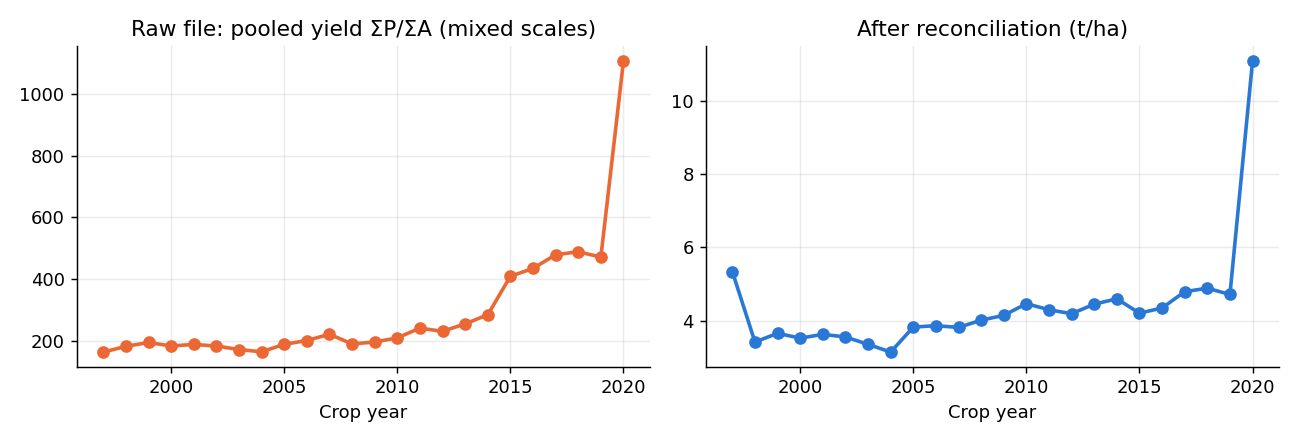
\includegraphics[width=0.9\textwidth]{fig1_stacked_source_fix.png}
  \caption{Pooled yield per year before and after the second release is removed.}
\end{figure}

\section{Model}
Notation: $x_c$ is the area (ha) given to crop $c$; $y_c$ is its average yearly yield (t/ha);
$a_c$ and $m_c$ are its smallest and largest yearly area. From the yearly totals over
districts, $A_t$ (area) and $P_t$ (production), over $n$ years:
\[
  y_c = \frac{1}{n}\sum_{t} \frac{P_t}{A_t}, \qquad
  a_c = \min_t A_t, \qquad
  m_c = \max_t A_t, \qquad
  h_c = \frac{1}{n}\sum_t A_t \ \text{(historical area)}.
\]

\textbf{Model 1 (maximise output):}
\[
  \max \sum_c y_c x_c \quad \text{s.t.} \quad \sum_c x_c \le L, \qquad a_c \le x_c \le m_c .
\]

\textbf{Model 2 (minimise land):}
\[
  \min \sum_c x_c \quad \text{s.t.} \quad \sum_c y_c x_c \ge D, \qquad a_c \le x_c \le m_c .
\]

By default $L = \sum_c h_c$ and $D = \sum_c y_c h_c$ (historical land and output).
The dual value of the land constraint, $\lambda^*$, is the extra output from one more hectare;
the dual of the target, $\mu^*$, is the extra land per extra tonne.

Model 1 is a continuous knapsack, so its solution has a simple structure:
\begin{enumerate}
  \item every crop gets its minimum area $a_c$;
  \item the remaining land goes to the highest-yield crop first, up to $m_c$, then the next;
  \item the crop where the land runs out is the single \emph{basic} crop, and its yield equals $\lambda^*$.
\end{enumerate}

Both models are solved with PuLP (CBC) and cross-checked with SciPy (HiGHS); the two agree
to within $10^{-9}$.

\section{Results (Karnataka, Kharif, 1998--2019)}
\textbf{Model 1}, at $L = 6{,}125{,}458$\,ha: $Z^* = 11.83$\,Mt ($+21.6\%$), $\lambda^* = 0.808$\,t/ha.
\begin{itemize}
  \item Expanded to the upper bound: Potato, Onion, Maize, Rice, Ragi, Jowar, Soyabean.
  \item Basic crop: Bajra (yield 0.81\,t/ha $= \lambda^*$).
  \item Held at the minimum: 11 lower-yield crops (pulses, oilseeds, millets).
\end{itemize}

\textbf{Model 2}, at $D = 9{,}729{,}947$\,t: minimum land 4.66\,Mha ($-23.9\%$),
$\mu^* = 0.3806$\,ha/t, basic crop Rice. Solving Model 1 at that land gives
$\lambda^* = 2.627$, and $1/\lambda^* = 0.3806 = \mu^*$, which confirms the duality between the models.

\begin{figure}[H]
  \centering
  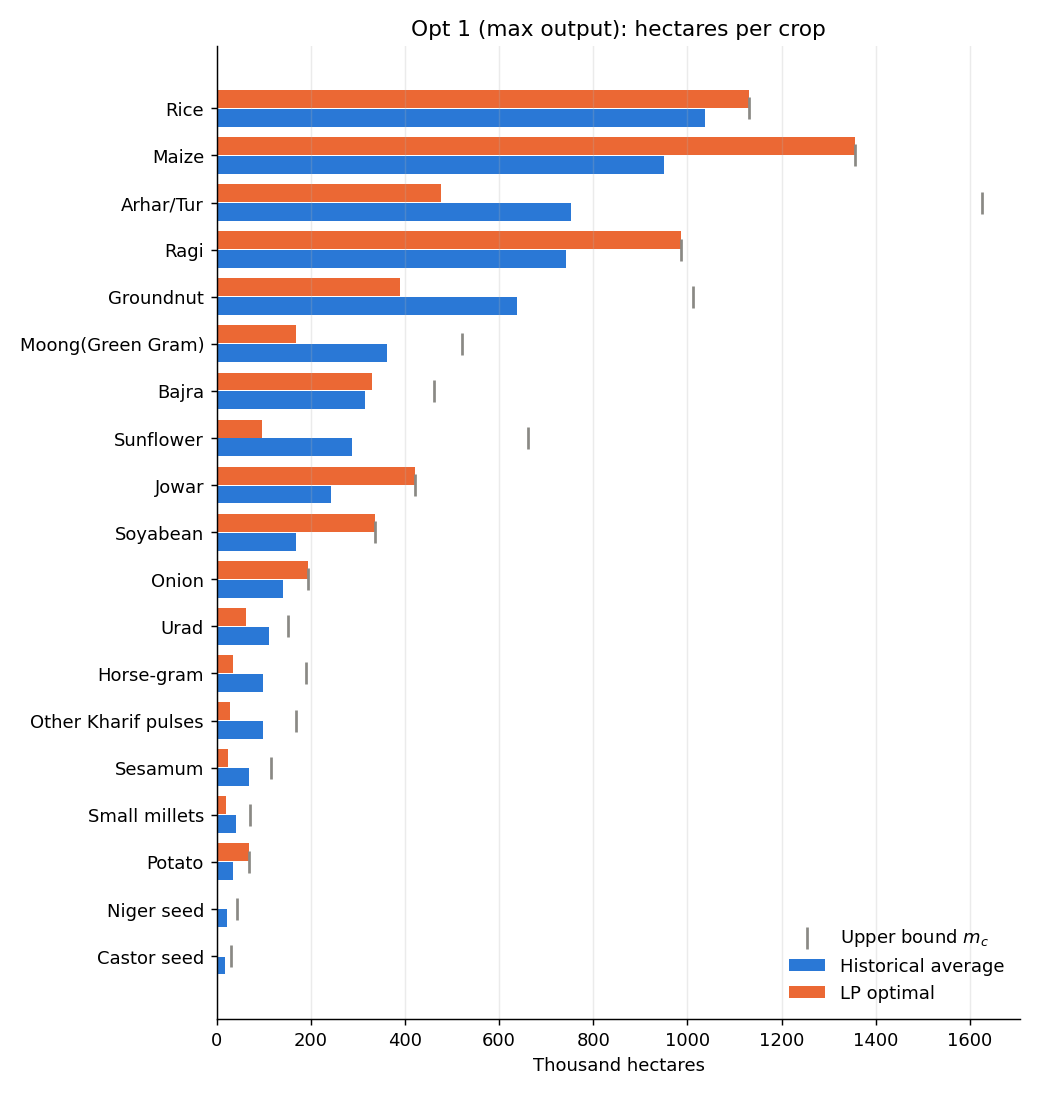
\includegraphics[width=0.85\textwidth]{fig3_opt1_allocation.png}
  \caption{Model 1 allocation compared with the historical area per crop.}
\end{figure}

\section{Sensitivity}
\begin{itemize}
  \item \textbf{More land:} $Z^*(L)$ is concave; $\lambda^*$ falls in steps
        ($6.6 \to 2.9 \to 1.6 \to 0.81 \to 0$) as each crop reaches its maximum area.
  \item \textbf{Yield ranging:} the plan holds while the expanded crops yield more than 0.81\,t/ha.
        Soyabean is closest to the margin: a fall of 0.05\,t/ha removes it from the expanded set.
  \item \textbf{Yield shocks:} a uniform $-30\%$ shock only rescales output (0\,ha moved);
        a $-30\%$ shock to Soyabean alone moves 288,406\,ha.
\end{itemize}

\begin{center}
\begin{tabular}{lrrrrr}
\toprule
Change allowed per crop ($\pm p\%$) & 5\% & 10\% & 20\% & 30\% & 50\% \\
\midrule
Output gain  & 3.1\% & 6.2\% & 12.5\% & 18.7\% & 31.2\% \\
Land saving  & 2.5\% & 5.0\% & 10.0\% & 15.0\% & 25.0\% \\
\bottomrule
\end{tabular}
\end{center}

A $\pm10\%$ band gives about 6\%, in line with the $+3.75$--$15\%$ reported by Supriya et al.\ (2022).

\begin{figure}[H]
  \centering
  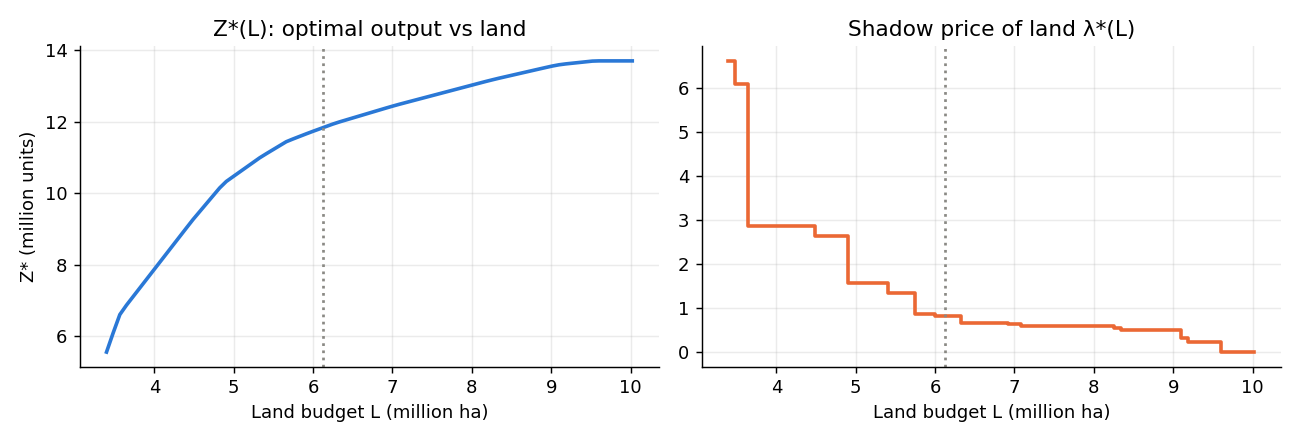
\includegraphics[width=0.85\textwidth]{fig5_parametric_land.png}
  \caption{Optimal output and $\lambda^*$ as the land budget changes.}
\end{figure}

\section{Multi-district comparison}
Both models were solved separately for each of the 27 districts. The median gain is
$+25.8\%$ output or $24.4\%$ less land.
\begin{itemize}
  \item Largest gains in the diverse dry north: Koppal ($+65\%$), Gadag ($+55\%$), Raichur ($+48\%$).
  \item Smallest gains in the coastal rice districts: Udupi ($+0.2\%$), Dakshina Kannada ($+0.6\%$).
  \item The gain rises with the number of crops grown ($r = 0.50$). Maize is the crop most often
        expanded (16 of 27 districts).
\end{itemize}

\begin{figure}[H]
  \centering
  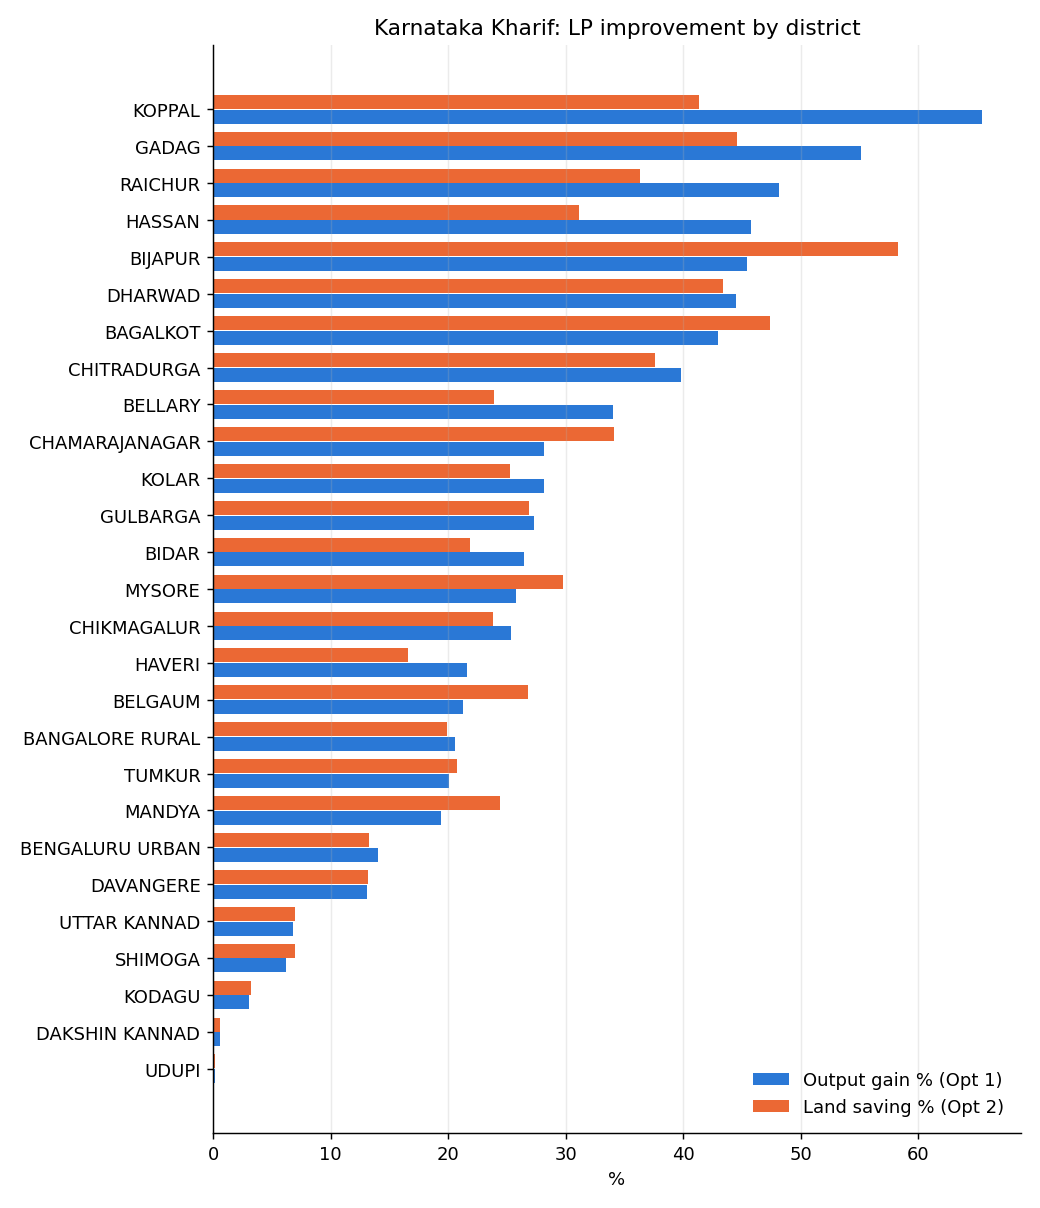
\includegraphics[width=0.9\textwidth]{fig7_multi_district.png}
  \caption{Output gain and land saving by district.}
\end{figure}

\section{Checking the results by changing the data}
The model can be tested by editing the data file, which has one line per record,
in any spreadsheet or text editor while the web app runs:
\begin{center}\small\texttt{Indian Agriculture Crop Production and yield (GOV)/Indian\_crop\_production\_yield\_dataset.csv}\end{center}
Within about 10 seconds of saving, the app reloads the file and re-solves.

\textbf{How an edit flows into the results.}
\begin{itemize}
  \item A line is added to its crop's yearly totals $A_t$ and $P_t$, so it changes that year's
        yield $P_t/A_t$ and therefore $y_c$ (one of 22 years).
  \item It changes a bound only if its year is the crop's smallest or largest year ($a_c$ or $m_c$).
  \item $Z^*$, the historical output and the gain change with $y_c$ and $h_c$. A crop at a bound
        keeps its hectares; the basic crop sets $\lambda^*$.
  \item A line is not used if it is outside 1998--2019, belongs to a crop counted in nuts or bales,
        belongs to a crop reported in too few years, or has a blank, zero or negative value.
\end{itemize}

\textbf{Tools in the app.}
\begin{itemize}
  \item \emph{Check the numbers by hand}: for one crop, the yearly totals, the formulas for
        $y_c$, $a_c$, $m_c$, $h_c$ with the numbers filled in, a check that they equal the values
        the LP uses, and the CSV lines behind each year.
  \item \emph{Look up a CSV line}: where a line goes (which crop-year total), or why it is not used.
  \item \emph{What the edit changed}: after a save, every coefficient and result that moved,
        before and after, with enough decimals to show even a very small change.
  \item \emph{Constraint check} on the results page: $\sum x_c \le L$, $\sum y_c x_c = Z^*$ and
        $a_c \le x_c \le m_c$, computed from the allocation table.
\end{itemize}

\textbf{Tests.}
\begin{itemize}
  \item For 50 sampled lines, a $+1\%$ edit and a deletion changed the results exactly for the
        40 lines the app marks as used, and not for the 10 it marks as unused (0 mismatches).
  \item Saving the file from LibreOffice Calc changed no value in any of the 358,657 lines.
\end{itemize}

Examples, all on line 82661 (Davangere, Maize, 2010), each applied after the previous one:
\begin{center}
\begin{tabular}{lll}
\toprule
Edit & Change shown by the app & Output gain \\
\midrule
Production $+20\%$ & $y_c$: $2.8551 \to 2.8602$ & $21.600\% \to 21.611\%$ \\
Area $+10\%$       & $h_c$: $+806.86$\,ha        & $21.611\% \to 21.583\%$ \\
Production $+1$\,t & $y_c$: $+3.9\times10^{-8}$; $Z^*$: $+0.053$\,t & $+8\times10^{-8}$ points \\
Line deleted       & $y_c$, $h_c$, $Z^*$ all change & $21.58\% \to 21.82\%$ \\
\bottomrule
\end{tabular}
\end{center}

\section{Web interface}
\texttt{python webapp/server.py} opens the interface at \texttt{http://127.0.0.1:8000}. It uses
the same code as this report, so the numbers are identical.
\begin{itemize}
  \item Any state and season can be chosen; seasons with fewer than two usable crops are shown
        but cannot be selected, with the reason.
  \item Model inputs: land available, production target, area limits, a minimum share of land
        under pulses, and the yield estimate (mean, median or area-weighted). Each slider shows
        the range in which the model has a solution.
  \item Model 1 is shown in green and Model 2 in brown throughout. The India and district maps
        can show either model and change smoothly when the inputs change.
\end{itemize}

\section{Limitations}
\begin{itemize}
  \item A tonne of onion counts the same as a tonne of pulses, so heavy crops are favoured.
  \item The area bounds drive the result: historical min--max bounds give $+21.6\%$,
        $\pm10\%$ bounds give $+6.2\%$.
  \item Prices, costs, soil, irrigation, labour, crop rotation and nutrition are not modelled.
\end{itemize}

\section{Conclusion}
Using public government data alone, re-planning Karnataka's Kharif crop mix could give
$+21.6\%$ output or $23.9\%$ land savings; a cautious $\pm10\%$ re-plan gives about 6\%.
Every number can be traced back to the data and checked by changing it. Next steps:
\begin{itemize}
  \item price- or nutrition-weighted objectives;
  \item crop rotation constraints;
  \item a stochastic LP using the yield variances already computed.
\end{itemize}

\section*{References}
\begin{enumerate}[label={[\arabic*]}]
  \item H.\,A.\ Taha, \emph{Operations Research: An Introduction}, 10th ed., Pearson, 2017.
  \item S.\ Wankhade and H.\ Lunge, LP technique for optimum resource allocation in agricultural production, Akola, 2012.
  \item F.\ Majeke et al., Linear programming approach: application in agriculture, 2020.
  \item S.\ Supriya et al., Optimal crop plans using LP in Jayashankar Bhupalpally district, Telangana, 2022.
  \item K.\,K.\ Paidipati and S.\,R.\ Padi, Optimal programming problems for crop planning, 2017.
  \item X.\ Liang, LP approach in agricultural production-land allocation, Springer, 2023.
  \item Ministry of Agriculture and Farmers Welfare, Government of India,
        \emph{District-wise, Season-wise Crop Production Statistics (1997--2020-21)}, data.gov.in.
\end{enumerate}

{\sloppy\textbf{Reproduce:} \texttt{python make\_clean\_data.py} builds the data file from the raw download;
\texttt{python run\_case\_study.py} regenerates every number and figure (tables in
\texttt{results/case\_study\_results.md}).\par}

\end{document}
